\documentclass[tikz,border=2pt]{standalone}
\usepackage{amsmath,amssymb}
\usepackage{tikz}
\usepackage{pgfplots}
\pgfplotsset{compat=1.18}

\begin{document}
% Phones: c1 = 170 below q = 35 units, c2 = 160 from 35 on; D = 2, K = 605, h = 5. The
% effective cost curve (thick) follows TCU1 below q and TCU2 from q on: cost 450 at y_m = 22
% versus 442.07 at the threshold 35, so order 35.
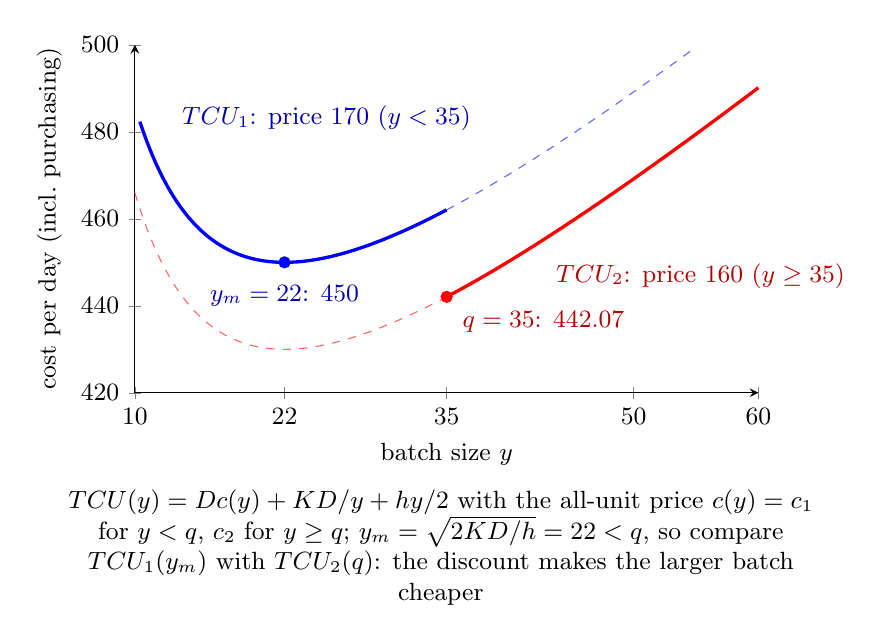
\begin{tikzpicture}
	\begin{axis}[width=9.5cm, height=6cm, xlabel={batch size $y$}, ylabel={cost per day (incl.\ purchasing)}, xmin=10, xmax=60, ymin=420, ymax=500, axis lines=left, clip=false, tick label style={font=\small}, label style={font=\small}, samples=100, xtick={10,22,35,50,60}]
		\addplot[blue!60, thin, dashed, domain=35:55] {340+1210/x+2.5*x};
		\addplot[red!60, thin, dashed, domain=10:35] {320+1210/x+2.5*x};
		\addplot[blue, very thick, domain=10.4:35] {340+1210/x+2.5*x};
		\addplot[red, very thick, domain=35:60] {320+1210/x+2.5*x};
		\addplot[only marks, mark=*, mark size=2pt, blue] coordinates {(22,450)};
		\addplot[only marks, mark=*, mark size=2pt, red] coordinates {(35,442.07)};
		\node[anchor=north, font=\small, blue!70!black] at (axis cs:22,447) {$y_m=22$: $450$};
		\node[anchor=north west, font=\small, red!70!black] at (axis cs:35.5,441) {$q=35$: $442.07$};
		\node[anchor=south west, font=\small, blue!70!black] at (axis cs:13,478) {$TCU_1$: price $170$ ($y<35$)};
		\node[anchor=north west, font=\small, red!70!black] at (axis cs:43,452) {$TCU_2$: price $160$ ($y\ge35$)};
	\end{axis}
	\node[anchor=north, font=\small, align=flush center, text width=9.6cm] at ([yshift=-2pt]current axis.outer south) {$TCU(y)=Dc(y)+KD/y+hy/2$ with the all-unit price $c(y)=c_1$ for $y<q$, $c_2$ for $y\ge q$; $y_m=\sqrt{2KD/h}=22<q$, so compare $TCU_1(y_m)$ with $TCU_2(q)$: the discount makes the larger batch cheaper};
\end{tikzpicture}
\end{document}
